\documentclass[smaller]{beamer}
\usetheme[english]{Berlin}
\usepackage{ngerman}
\useoutertheme{infolines}
\beamertemplatenavigationsymbolsempty
\setbeamertemplate{caption}[numbered]
\usepackage{pgfplots,tikz,subfigure}
\usepackage{amsmath,amsthm}
\usepackage{hyperref,graphics,graphicx,color,algorithm,algorithmic,enumerate}
\usepackage{mymacros,wrapfig,relsize}
\usepackage{pict2e}
\usepackage[utf8x]{inputenc}

\newcommand{\ri}{\mathrm{i}}
\newcommand{\T}{\mathsf{T}}
\renewcommand{\H}{\mathsf{H}}
\newcommand{\eps}{\varepsilon}
\newcommand{\To}{\rightarrow}
\newcommand{\sddots}{\scalebox{0.6}{$\ddots$}}
\usepackage[pdf]{pstricks}
\usepackage{sansmathfonts}
\usepackage{eurosym}
\usepackage{ulem}
%\usepackage{arev}
%\renewcommand\familydefault{\sfdefault}

\DeclareMathOperator{\loc}{loc}
\DeclareMathOperator{\rank}{rank}
\DeclareMathOperator{\RE}{Re}
\DeclareMathOperator{\IM}{Im}
\DeclareMathOperator{\In}{In}
\DeclareMathOperator{\im}{im}
\DeclareMathOperator{\Gl}{Gl}
\DeclareMathOperator{\spa}{span}
\DeclareMathOperator{\ext}{{ext}}
\DeclareMathOperator{\ind}{ind}
\DeclareMathOperator{\normalrank}{normalrank}
\DeclareMathOperator{\essup}{ess\,sup}
\DeclareMathOperator{\vect}{vec}

\newcommand{\re}{\mathrm{e}}
\newcommand{\ddt}{\tfrac{\mathrm{d}}{\mathrm{d}t}}
\newcommand{\sys}[4]{\left[\begin{array}{c|c} #1 & #2 \\ \hline #3 & #4 \end{array}\right]}

\renewcommand{\tilde}{\widetilde}
\renewcommand{\hat}{\widehat}


\title[]{Optimierung f\"ur Studierende der Informatik}
\subtitle{-- 8. Vorlesung --}
\author[Matthias Voigt]{\textbf{Matthias Voigt$^{1,2}$}}
\institute[]{
\begin{columns}
%\begin{center}
\column{0.45\textwidth}{\centering {$^1$Universit\"at Hamburg \\ Fachbereich Mathematik \\ Hamburg \\ }}
\column{0.45\textwidth}{\centering {$^2$Technische Universit\"at Berlin \\ Institut f\"ur Mathematik \\ Berlin  \\}}
%\end{center}
\end{columns}
}
\date[]{Universit\"at Hamburg
\begin{columns}
\column{0.45\textwidth}{\centering 
\includegraphics[width = 1.2\textwidth]{uhh-logo.png}\\}
\end{columns}
}

\definecolor{tucgreen}{rgb}{0.0,0.5,0.27}
\definecolor{tucred}{rgb}{0.75,0,0}
\definecolor{tucorange}{rgb}{1.0,.5625,0}
\definecolor{mpired}{HTML}{990000}
\definecolor{mpigreen}{HTML}{5C871D}
\definecolor{mpiblue}{HTML}{006AA9}
\definecolor{mpibg1}{HTML}{5D8B8A}
\definecolor{mpibg2}{HTML}{BFDFDE}
\definecolor{mpibg3}{HTML}{A7C1C0}
\definecolor{mpibg4}{HTML}{7DA9A8}
\definecolor{mpigrey}{rgb}{0.9294,0.9294,0.8784}

\begin{document}

\maketitle

\begin{frame}
 \frametitle{Matchings und Knotenüberdeckungen in bipartiten Graphen}
 In diesem Abschnitt geht es größtenteils um eine Anwendung der Ergebnisse über Maximalflüsse auf \alert{ungerichtete} Graphen. \\ \vspace*{0.2cm}
 
 Wir wiederholen zunächst einmal die Definition eines ungerichteten Graphen, die bereits aus den Grundvorlesungen bekannt ist. \\ \vspace*{0.2cm} 
\textbf{Definition:} Ein \structure{ungerichteter Graph} $G$ ist ein Paar $(V,E)$, wobei $V$ eine beliebige endliche Menge und $E$ eine Teilmenge der Menge aller zweielementigen Teilmengen von $V$ ist. Man nennt $V$ die \structure{Knotenmenge} und $E$ die \structure{Kantenmenge} von $G$.
\end{frame}

\begin{frame}
 \frametitle{Ein Beispiel}
 \textbf{Beispiel:}
\begin{align*}
V &= \{ 1, 2, 3, 4, 5, 6 \} \\
E &= \big\{ \{ 1,2 \},\ 
\{ 2,3 \},\ 
\{ 3,4 \},\ 
\{ 4,5 \},\ 
\{ 1,5 \},\ 
\{ 3,5 \},\ 
\{ 1,6 \},\ 
\{ 2,6 \},\ 
\{ 3,6 \},\ 
\{ 5,6 \} \big\}
\end{align*}

Den Graphen dieses Beispiels kann man wie folgt darstellen:

\begin{center}
 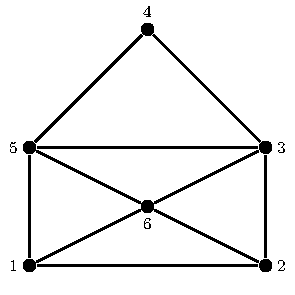
\includegraphics{fig33.pdf}
\end{center}
\end{frame}

\begin{frame}
 \frametitle{Matchings und bipartite Graphen}
 Wir setzen die in {\glqq}Mathematik I (DM){\grqq} behandelten Grundbegriffe über Graphen und die dort verwendeten Schreibweisen als bekannt voraus. \\ \vspace*{0.2cm}

In der Überschrift dieses Abschnitts kommen die beiden Begriffe {\glqq}Matching{\grqq} und {\glqq}bipartiter Graph{\grqq} vor. Im Folgenden werden diese beiden Begriffe definiert und erläutert. \\ \vspace*{0.2cm}

\textbf{Definition:} Es sei $G=(V,E)$ ein (ungerichteter) Graph. Eine Teilmenge $M$ von $E$ wird ein \structure{Matching} von $G$ genannt, falls je zwei verschiedene Kanten von $M$ niemals einen Knoten gemeinsam haben. \\ \vspace*{0.2cm}

Wir wollen hier die folgende \alert{Konvention} verwenden: Liegt ein ungerichteter Graph vor, so kann das Adjektiv {\glqq}ungerichtet{\grqq} auch wegfallen; liegt hingegen ein gerichteter Graph vor, so soll das Adjektiv {\glqq}gerichtet{\grqq} nicht weggelassen werden. \\ \vspace*{0.2cm}

In der folgenden Skizze wird ein Graph $G$ und ein Matching $M$ von $G$ dargestellt: 
\end{frame}

\begin{frame}
 \frametitle{Ein Matching $M$ von $G$}
 \begin{center}
  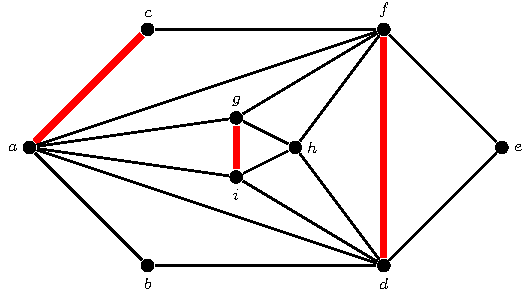
\includegraphics[scale=0.8]{fig34.pdf}
 \end{center}
Die Kanten von $M$ wurden fett und rot gezeichnet. $M$ besteht aus drei Kanten:
\[
M = \big\{ \{ a,c \},\ \{ g,i \},\ \{ d,f \} \big\}.
\]
Können Sie ein Matching mit mehr als drei Kanten angeben? \\ \vspace*{0.2cm}

\textbf{Zur Übung:} Geben Sie einen zusammenhängenden Graphen $G$ mit 10 Kanten an, für den gilt: Es gibt in $G$ ein Matching $M$ mit $|M| = 2$, aber ein Matching mit mehr als 2 Kanten gibt es nicht.
\end{frame}

\begin{frame}
 \frametitle{Die Matchingzahl}
 \textbf{Definition:}
Die \structure{Matchingzahl} $m(G)$ eines Graphen $G$ wird definiert durch:
\[
m(G) = \max{\big\{ |M| : M \text{ ist ein Matching von $G$} \big\}}.
\]

Für den oben abgebildeten Graphen $G$ mit $V(G) = \bigl\{ a,\ldots,i \bigr\}$ gilt $m(G) = 4$. \\ \vspace*{0.2cm}

Unter dem \structure{Matching-Problem} versteht man das Problem, für einen gegebenen Graphen $G$ ein Matching $M$ mit größtmöglicher Kantenzahl zu finden; mit anderen Worten: Gesucht ist ein Matching $M$, für das
\[
|M| = m(G)
\] 
gilt. \\ \vspace*{0.2cm}

Wir werden das \alert{Matching-Problem für bipartite Graphen} behandeln. Zunächst einmal ist die noch ausstehende Definition eines bipartiten Graphen zu geben.
\end{frame}

\begin{frame}
\frametitle{Bipartite Graphen}
\textbf{Definition:} Ein Graph $G=(V,E)$ heißt \structure{bipartit}, falls seine Knotenmenge $V$ in zwei disjunkte Teilmengen $X$ und $Y$ zerlegt werden kann, so dass jede Kante von $G$ einen Knoten aus $X$ mit einem Knoten aus $Y$ verbindet.\\ \vspace*{0.2cm}

Kanten sollen also immer nur zwischen den Mengen $X$ und $Y$ verlaufen, aber \alert{niemals innerhalb von $X$ oder innerhalb von $Y$}. \\ \vspace*{0.2cm}

Hier ein \textbf{Beispiel} eines bipartiten Graphen:
\begin{center}
 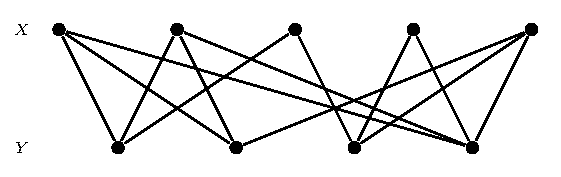
\includegraphics{fig35.pdf}
\end{center}
\end{frame}

\begin{frame}
 \frametitle{Zuordnung von Personen zu Jobs}
 Bipartite Graphen sowie Matchings in bipartiten Graphen treten besonders häufig in Situationen auf, in denen es um die Zuordnung von Personen oder Objekten zu anderen Personen oder Objekten geht -- wie etwa im nachfolgenden Problem. \\ \vspace*{0.2cm}

Gegeben seien $m$ Personen und $n$ Jobs\index{Job}. Die Personen seien mit $x_1,\ldots,x_m$ und die Jobs mit $y_1,\ldots,y_n$ bezeichnet. Ist eine Person $x_i$ für einen Job $y_j$ geeignet, so ziehen wir eine Kante von $x_i$ nach $y_j$, wie beispielsweise im folgenden Graphen:
\begin{center}
 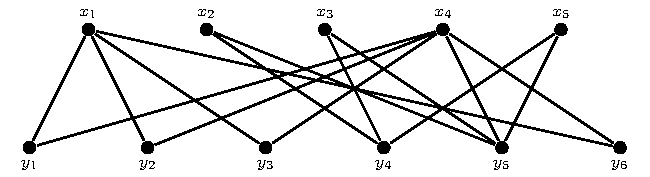
\includegraphics{fig36.pdf}
\end{center}
\end{frame}

\begin{frame}
 \frametitle{Perfekte Matchings}
 Die Aufgabe ist nun, möglichst vielen Personen einen Job zu geben, wobei Jobs jedoch nur mit geeigneten Personen zu besetzen sind; außerdem soll kein Job mehrfach vergeben werden und keine Person soll mehr als einen Job erhalten. \\ \vspace*{0.2cm}

Perfekt wäre es natürlich, wenn jede Person einen Job bekäme und auch kein Job unbesetzt bliebe. In diesem Fall spricht man von einem \structure{perfekten Matching}. Auch wenn es um nicht-bipartite Graphen geht, spricht man von perfekten Matchings. \\ \vspace*{0.2cm}

Der Deutlichkeit halber sei noch einmal die genaue Definition gegeben. \\ \vspace*{0.2cm}

\textbf{Definition:} Es sei $G=(V,E)$ ein Graph. Ein Matching $M$ von $G$ heißt \structure{perfekt}, falls es zu jedem Knoten $v$ von $G$ eine Kante $e \in M$ gibt, die $v$ trifft.
\end{frame}

\begin{frame}
 \frametitle{Ein Graph mit perfektem Matching}
 Zur Illustration ein Graph $G$, der ein perfektes Matching  besitzt:

\begin{center}
 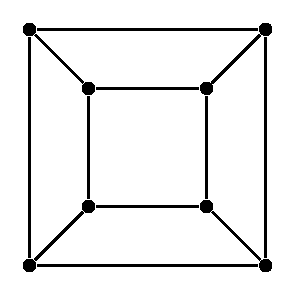
\includegraphics{fig37.pdf}
\end{center}

\textbf{Klar ist:} Besitzt ein Graph $G=(V,E)$ ein perfektes Matching, so ist $|V|$ eine gerade Zahl und es gilt
\[
m(G) = \frac{|V|}{2}.
\]
\end{frame}

\begin{frame}
\frametitle{Eine Übungsaufgabe}
\textbf{Zur Übung:} Besitzt der folgende Graph ein perfektes Matching?
\begin{center}
 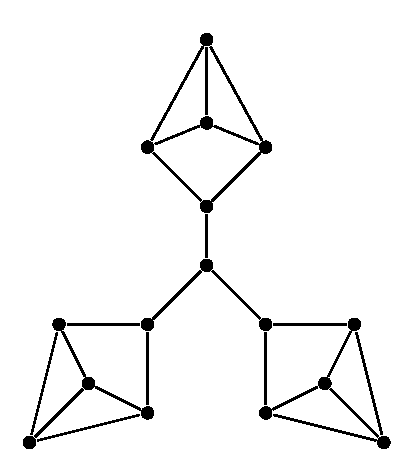
\includegraphics[scale = 0.8]{fig38.pdf}
\end{center}
\end{frame}

\begin{frame}
 \frametitle{Das Matching-Problem für bipartite Graphen}
 Nach diesem einführenden Teil kommen wir nun wie angekündigt zum \alert{Matching-Problem für bipartite Graphen}. Wir folgen dabei zum Teil der Darstellung im folgenden Lehrbuch:
\begin{itemize}
\item Jon Kleinberg, Éva Tardos: \textit{Algorithm Design}. Pearson (2006).
\end{itemize} \vspace*{0.2cm}

\textbf{Das Problem:} \\ \vspace*{0.2cm}

\alert{Eingabe:} ein bipartiter Graph $G=(V,E)$ mit zugehöriger Knotenpartition $V = X \cup Y$. \\ \vspace*{0.2cm}

\alert{Gesucht:} ein Matching von $G$ mit maximaler Anzahl von Kanten. \\ \vspace*{0.2cm}

Wir setzen im Folgenden stets voraus, dass der betrachtete bipartite Graph $G$, für den ein Matching mit maximaler Kantenzahl gefunden werden soll, keine Knoten vom Grad 0 (\alert{{\glqq}isolierte Knoten{\grqq}}) besitzt; dies ist möglich, da isolierte Knoten für das Matching-Problem offenbar keine Rolle spielen.
\end{frame}

\begin{frame}
 \frametitle{Der Algorithmus}
 Es soll der \alert{Netzwerk-Fluss-Algorithmus} von Edmonds und Karp angewendet werden, um das Matching-Problem für bipartite Graphen zu lösen. Netzwerk-Fluss-Algorithmen lassen sich auf \alert{gerichtete} Graphen anwenden, beim Matching-Problem geht es jedoch um \alert{ungerichtete} Graphen; außerdem brauchen wir eine \alert{Quelle} $s$, eine \alert{Senke} $t$ und \alert{Kapazitäten}. \\ \vspace*{0.2cm}

Dies alles stellt keine Schwierigkeit dar, da wir einen gegebenen bipartiten Graphen in ein passendes Netzwerk überführen können.
\end{frame}

\begin{frame}
 \frametitle{\"Uberführung in ein Netzwerkproblem}
 Es sei $G=(V,E)$ ein bipartiter Graph mit Knotenpartition $V=X \cup Y$. Wir bilden auf folgende Art ein \alert{Flussnetzwerk:}
\begin{itemize}
\item Alle Kanten von $G$ werden von $X$ nach $Y$ gerichtet.
\item Wir fügen zwei neue Knoten $s$ und $t$ hinzu und verbinden $s$ mit jedem Knoten $x \in X$ durch die (gerichtete) Kante $(s,x)$; analog: Zu jedem $y \in Y$ wird die Kante $(y,t)$ hinzugefügt.
\item Jede Kante erhält die Kapazität 1.
\end{itemize} \vspace*{0.2cm}

Den so aus $G$ entstandenen gerichteten Graphen wollen wir $G'$ nennen; das entstandene Netzwerk ist also
\[
N = \big( G', c, s, t \big)
\]\label{page:11:6}
mit $c(e)=1$ für alle Kanten $e$ von $G'$.
\end{frame}

\begin{frame}
\frametitle{Der Algorithmus}
\textbf{Illustration dieser Konstruktion:}
\begin{center}
 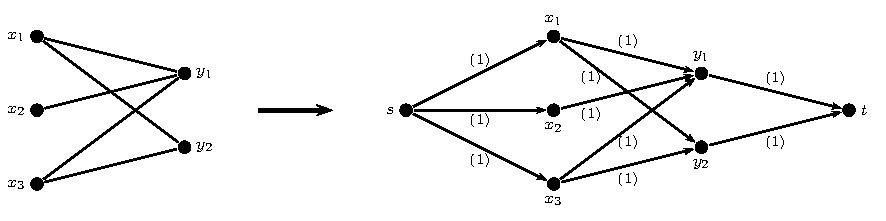
\includegraphics[scale=0.8]{fig39.pdf}
\end{center}

\alert{Der angekündigte Algorithmus zur Berechnung eines Matchings von $G$ mit maximaler Kantenzahl ist sehr einfach: Er besteht lediglich darin, dass man mit dem Algorithmus von Edmonds und Karp einen maximalen Fluss $f^*$ von $N$ berechnet}. \\ \vspace*{0.2cm} Wir werden sehen (siehe Analyse des Algorithmus), dass es ebenfalls ganz einfach ist, aus dem erhaltenen Maximalfluss $f^*$ das gewünschte Matching zu gewinnen.
\end{frame}

\begin{frame}
 \frametitle{Analyse des Algorithmus}
 Wir erinnern uns zunächst an eine \alert{Besonderheit des Netzwerk-Fluss-Problems}, die sich in unserem Zusammenhang als entscheidend erweist:
\begin{quote}
%\label{eq:11:*}
%\tag{$\star$}
%\begin{array}{c}
\alert{Setzt man -- wie wir es immer gemacht haben -- voraus, dass alle Kapazitäten ganzzahlig sind, so gibt es auch immer einen ganzzahligen Maximalfluss: Der Ford-Fulkerson-Algorithmus liefert bei ganzzahligen Kapazitäten auch immer einen ganzzahligen Maximalfluss.}
%\end{array}
\end{quote}
Wenn Sie sich noch einmal von der Richtigkeit dieser Feststellung überzeugen wollen: Ein kurzer Blick in Vorlesung 6 sollte genügen. Da die getroffenen Feststellungen für den Ford-Fulkerson-Algorithmus gelten, gelten sie natürlich ebenfalls für den Algorithmus von Edmonds und Karp.
\end{frame}

\begin{frame}
 \frametitle{Analyse des Algorithmus}
 Nun zur \textbf{Analyse unseres Matching-Algorithmus}: \alert{Diese basiert auf dem Nachweis, dass sich Matchings in $G$ und ganzzahlige Flüsse in $N = (G',c,s,t)$ auf eine leicht durchschaubare Art entsprechen}.

\begin{enumerate}[I)]
\item Nehmen wir zunächst an, dass ein Matching $M$ von $G$ gegeben ist, das -- sagen wir -- aus $k$ Kanten $\big\{ x_{i_1}, y_{i_1}\big\}, \ldots, \big\{ x_{i_k}, y_{i_k} \big\}$ besteht. Dann gehört zu $M$ ein ganzzahliger Fluss $f$ auf $N$, der wie folgt definiert wird:
\[
\begin{array}{c}
f(s, x_{i_j}) = f(x_{i_j}, y_{i_j}) = f(y_{i_j}, t) = 1 \quad (j = 1,\ldots,k), \\[2mm]
f(e) = 0 \quad \text{sonst.}
\end{array}
\]

Man erkennt sofort, dass es sich hierbei um einen Fluss handelt, dass also 1) und 2) aus der Definition eines Flusses erfüllt sind; außerdem gilt $w(f) = k$.
\end{enumerate}
\end{frame}

\begin{frame}
\frametitle{Analyse des Algorithmus}
\begin{enumerate}[I)]
\setcounter{enumi}{1}
\item Nun wollen wir umgekehrt annehmen, dass ein ganzzahliger Fluss $f$ auf $N$ gegeben ist, für den $w(f)=k$ gilt. Aufgrund von 1) gilt dann
\[
0 \leq f(e) \leq c(e) = 1
\]

für alle Kanten $e$ von $G'$. Hieraus folgt wegen der Ganzzahligkeit von $f$, dass für jede Kante $e$ von $G'$
\[
f(e) = 0 \quad \text{oder} \quad f(e) = 1
\]

gilt. Wir definieren nun $M'$ als die Menge derjenigen (gerichteten) Kanten $e$ von $G'$, für die gilt: $e$ führt von $X$ nach $Y$ und es gilt $f(e)=1$. 
\end{enumerate}
\end{frame}

\begin{frame}
 \frametitle{Drei Feststellungen}
 Im Buch von Kleinberg und Tardos werden drei einfache Fakten über die Menge $M'$ bewiesen. Wir schauen uns diese besonders wichtigen Feststellungen an: \\ \vspace*{0.2cm}

\begin{enumerate}[i)]
\item \alert{$M'$ enthält $k$ Kanten.} \\

\textbf{Beweis:} Betrachte den Schnitt $(A, B)$ in $G'$ mit $A = \big\{s\big\} \cup X$. Der Wert des Flusses ist $w(f) = f^+(A) - f^-(A)$\footnote{Vgl. Vorlesung 6 (Stichwort: \alert{Nettofluss}).}. Allerdings ist $f^+(A) = |M'|$, denn die Kanten in $M'$ verlassen $A$ und für jede Kante $e$ in $M'$ gilt $f(e) = 1$; weiter ist $f^-(A) = 0$, da es keine Kanten gibt, die von $B$ nach $A$ zeigen. Deshalb enthält $M'$ $k$ Kanten. \qquad $\Box$

\item \alert{Jeder Knoten in $X$ ist Startknoten höchstens einer Kante in $M'$.} \\

\textbf{Beweis:} Sei $x \in X$ der Startknoten mindestens zweier Kanten in $M'$. Da unser Fluss ganzzahlig ist, verlassen $x$ mindestens zwei Einheiten des Flusses. Durch die Flusserhaltung müssen allerdings mindestens zwei Einheiten des Flusses nach $x$ hineinfliessen. Dies ist ein Widerspruch, da nur eine Kante mit der Kapazität 1 nach $x$ zeigt. \qquad $\Box$

\item \alert{Jeder Knoten in $Y$ ist der Endknoten höchstens einer Kante in $M'$.} \\
\textbf{Beweis:} Analog zu ii). \qquad $\Box$
\end{enumerate}
\end{frame}

\begin{frame}
 \frametitle{Zusammenfassung}
 Bei den Kanten von $M'$ handelt es sich um gerichtete Kanten, die von $X$ nach $Y$ führen. Mit $M$ wollen wir die dazugehörige Menge von ungerichteten Kanten bezeichnen. Aufgrund von i), ii) und iii) gilt dann: \alert{$M$ ist ein Matching von $G$ mit $|M|=k$}. \\ \vspace*{0.2cm}

\textbf{Zusammenfassung von I) und II):} In I) haben wir gesehen, dass es zu jedem Matching $M$ von $G$ mit $|M|=k$ einen ganzzahligen Fluss $f$ in $N$ mit $w(f)=k$ gibt. In II) haben wir erkannt, dass es umgekehrt zu jedem ganzzahligen Fluss $f$ in $N$ mit $w(f)=k$ ein Matching $M$ von $G$ mit $|M|=k$ gibt. Ist $f^*$ ein ganzzahliger Maximalfluss auf $N$, so gilt also
\[
w(f^*) = m(G).
\]

Außerdem haben wir in II) gesehen, wie man ein Matching $M$ von $G$ mit $|M|=m(G)$ erhält, wenn ein ganzzahliger Maximalfluss $f^*$ von $N$ vorliegt: Man hat nichts weiter zu tun, als die Menge $M'$ derjenigen Kanten $e$ von $G'$ zu betrachten, die von $X$ nach $Y$ führen und für die $f^*(e)=1$ gilt; um $M$ mit $|M| = m(G)$ zu erhalten, braucht man nur noch die Orientierung dieser Kanten wegzulassen.
\end{frame}

\begin{frame}
 \frametitle{Komplexität}
$G=(V,E)$ sei bipartit mit $|V|=n$ und $|E|=m$; isolierte Knoten soll es in $G$ nicht geben. \\ \vspace*{0.2cm}

\alert{Beobachtung:} Jede Kante in $G'$ hat die Kapazität 1. Die Summe der Kapazitäten der an $s$ stoßenden Kanten ist demnach gewiss nicht größer als $n$. Für jeden ganzzahligen Maximalfluss $f^*$ von $N$ gilt deshalb $w(f^*) \leq n$. Folglich benötigt der Algorithmus von Edmonds und Karp nicht mehr als $n$ Iterationen, um einen Maximalfluss in $N=(G',c,s,t)$ zu finden. \\ \vspace*{0.2cm}

Anknüpfend an diese Beobachtung lässt sich zeigen, dass Folgendes gilt (Details siehe Kleinberg/Tardos): Der Algorithmus von Edmonds und Karp kann benutzt werden, um in einem bipartiten Graphen ein Matching maximaler Größe in $O(nm)$ Zeit zu finden. 
\end{frame}

\begin{frame}
 \frametitle{Alternierende und augmentierende Pfade}
 \alert{Es ist lohnend, sich genauer anzuschauen, wie flussvergrößernde Pfade im Falle des bipartiten Matching-Problems konkret aussehen}. Hierzu schauen wir uns den folgenden bipartiten Graphen $G$ an; die Kanten $\bigl\{ x_2,y_2 \bigr\}$, $\bigl\{ x_3,y_3 \bigr\}$ und $\bigl\{ x_5,y_5 \bigr\}$ bilden ein Matching $M$ in $G$. (Hier und im Folgenden sind Matchingkanten, d.h. Kanten aus $M$, immer durch Wellenlinien dargestellt.)

\begin{center}
 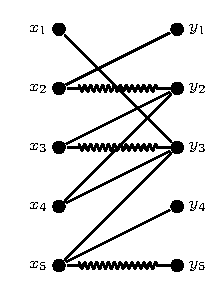
\includegraphics{fig40.pdf}
\end{center}
\end{frame}

\begin{frame}
 \frametitle{Ein flussvergrößernder Pfad}
 Es sei $f$ der ganzzahlige Fluss in $N=(G',c,s,t)$, der $M$ entspricht (vgl. I)). Da $|M|$ nicht größtmöglich ist, ist $f$ kein Maximalfluss und folglich muss es einen flussvergrößernden $s,t$-Pfad geben. Beispielsweise ist der folgende Pfad $P'$ ein flussvergrößernder Pfad in $N=(G',c,s,t)$:
\[
P':\quad s,\ x_4,\ y_3,\ x_3,\ y_2,\ x_2,\ y_1,\ t.
\]

\begin{center}
 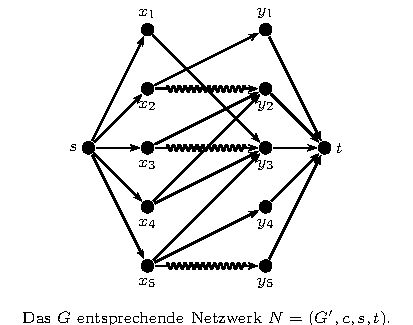
\includegraphics[scale=0.9]{fig41.pdf}
\end{center}
\end{frame}

\begin{frame}
\frametitle{Der entsprechende ungerichtete Pfad}
 
\alert{Wir wissen:} Alle Kapazitäten von $N$ sind gleich 1. Deshalb konnte in der Abbildung, in der $N$ dargestellt wird, auf die Angabe der Kapazitäten verzichtet werden. Außerdem: Für neun gerichtete Kanten $e$ gilt $f(e)=1$ (Für welche nämlich?); für die übrigen Kanten gilt $f(e)=0$. \\ \vspace*{0.2cm}

Dem Pfad $P'$ entspricht in $G$ ein ungerichteter Pfad, den wir $P$ nennen wollen.
\[
P:\quad x_4,\ y_3,\ x_3,\ y_2,\ x_2,\ y_1.
\]

Man beachte, dass sich auf $P$ Kanten, die nicht in $M$ sind, mit Kanten aus $M$ abwechseln:

\begin{center}
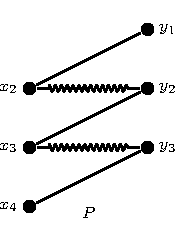
\includegraphics{fig42.pdf}
\end{center}
\end{frame}

\begin{frame}
 \frametitle{Der entsprechende ungerichtete Pfad}
 Dasselbe, nur ein wenig anders formuliert: \alert{Auf $P$ wechseln sich Nicht-Matchingkanten mit Matchingkanten ab}. Außerdem beginnt $P$ in einem Knoten von $X$, der in $G$ \alert{ungepaart} ist, d.h., es gibt im gesamten Graphen $G$ keine Matchingkante, die an diesen Knoten stößt. Und schließlich gilt: $P$ endet in einem Knoten von $Y$, der in $G$ ebenfalls ungepaart ist. \\ \vspace*{0.2cm}

Vergrößert man nun wie üblich den Fluss $f$ mithilfe von $P'$, so erkennt man, dass dies nichts anderes bedeutet, als das Matching $M$ folgendermaßen mithilfe von $P$ zu vergrößern: \\ \vspace*{0.2cm}

\begin{quote}
\alert{Man entfernt aus $M$ alle Matchingkanten von $P$ und nimmt stattdessen die Nicht-Matchingkanten von $P$ hinzu}.
\end{quote}\label{page:11:5}
\end{frame}

\begin{frame}
 \frametitle{Austausch von Matching- und Nicht-Matchingkanten entlang $P$}
 Kurz gesagt: \alert{Man nimmt längs $P$ einen Austausch von Matching- und Nicht-Matchingkanten vor}. \\ \vspace*{0.2cm}

Dass dies so schön funktioniert, liegt natürlich an den drei bereits oben genannten Eigenschaften von $P$:

\begin{enumerate}[1.]
\item Auf $P$ wechseln sich Nicht-Matchingkanten mit Matchingkanten ab;
\item $P$ beginnt in einem ungepaarten Knoten von $X$; 
\item $P$ endet in einem ungepaarten Knoten von $Y$.
\end{enumerate}

Besitzt ein Pfad $P$ die Eigenschaften 1.--3., so nennt man $P$ einen \structure{augmentierenden Pfad}\label{page:11:3}. Wir haben gesehen, wozu augmentierende Pfade gut sind: \alert{Mit ihrer Hilfe lässt sich aus einem gegebenen Matching $M$ ein Matching mit $|M|+1$ Kanten gewinnen.} \\ \vspace*{0.2cm}
Es lässt sich unschwer beweisen, dass einem flussvergrößernden Pfad in $N=(G',c,s,t)$ immer ein augmentierender Pfad in $G$ entspricht (und umgekehrt). Da dies eine wichtige Feststellung ist, halten wir das Gesagte noch einmal fest:
\end{frame}

\begin{frame}
 \frametitle{Feststellung 1}
 \textbf{Feststellung 1:} Es sei $G=(V,E)$ ein bipartiter Graph mit Knotenpartition $V = X \cup Y$; es gelte $X=\big\{ x_1,\ldots,x_m\big\}$ und $Y = \big\{ y_1,\ldots,y_n \big\}$. Ferner sei $N=(G',c,s,t)$ das zu $G$ gehörige Flussnetzwerk. Es sei ein Matching $M$ von $G$ gegeben und $f$ sei der zu $M$ gehörige ganzzahlige Fluss in $N$. Dann gilt:
\begin{enumerate}[i)]
\item Ist $P' = (s,x_{i_1},y_{i_1},\ldots,x_{i_k},y_{i_k},t)$ ein flussvergrößernder Pfad in $N$, so ist $P = (x_{i_1},y_{i_1},\ldots,x_{i_k},y_{i_k})$ ein augmentierender Pfad in $G$.
\item Ist umgekehrt $P = (x_{i_1},y_{i_1},\ldots,x_{i_k},y_{i_k})$ ein augmentierender Pfad in $G$, so ist $P' = (s,x_{i_1},y_{i_1},\ldots,x_{i_k},y_{i_k},t)$ ein flussvergrößernder Pfad in $N$.
\end{enumerate} \vspace*{0.2cm}
Neben dem Begriff des augmentierenden Pfads spielt der Begriff eines
\begin{center}
	\alert{alternierenden Pfads}
\end{center}
eine zentrale Rolle.
\end{frame}

\begin{frame}
 \frametitle{Alternierende Pfade}
 \textbf{Definition:}
Gegeben sei ein bipartiter Graph $G=(V,E)$ mit dazugehöriger Knotenpartition $V=X \cup Y$. Außerdem sei ein Matching $M$ von $G$ gegeben. Ein Pfad $P$ in $G$ wird \structure{alternierender Pfad} genannt, wenn er in einem ungepaarten Knoten $x$ von $X$ beginnt und wenn Folgendes gilt: $P$ besteht entweder nur aus $x$ oder auf $P$ wechseln sich Nicht-Matchingkanten mit Matchingkanten ab.

\begin{center}
 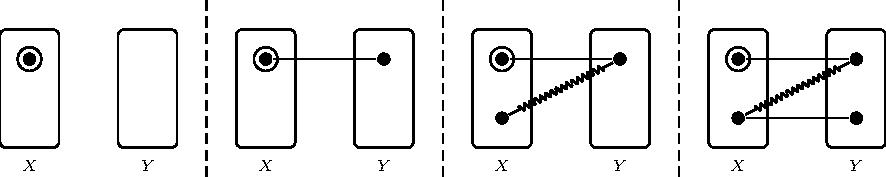
\includegraphics[scale=0.8]{fig43.pdf}
\end{center}
Die Zeichnung stellt alternierende Pfade der Längen 0, 1, 2 und 3 dar; ungepaarte Knoten sind durch einen umkreisten Punkt gekennzeichnet und Matchingkanten durch Wellenlinien.
\end{frame}

\begin{frame}
 \frametitle{Alternierende und augmentierende Pfade}
 Man beachte, dass jeder augmentierende Pfad auch ein alternierender Pfad ist: \alert{Augmentierende Pfade sind also spezielle alternierende Pfade}. Die nachfolgende Zeichnung stellt einen augmentierenden Pfad der Länge 5 dar:

\begin{center}
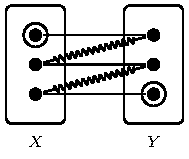
\includegraphics[scale=0.9]{fig44.pdf}
\end{center}

In Feststellung 1 haben wir festgehalten, dass sich augmentierende Pfade in $G$ und flussvergrößernde Pfade in $N$ auf eine ganz einfache Art entsprechen. \alert{Eine analoge Feststellung lässt sich auch für alternierende Pfade treffen}. Dies wird im Folgenden ausgeführt. \\ \vspace*{0.2cm}

Der Unterschied zwischen den Begriffen {\glqq}augmentierender Pfad{\grqq} und {\glqq}alternierender Pfad{\grqq} besteht darin, dass augmentierende Pfade immer in einem ungepaarten Knoten von $Y$ enden, während alternierende Pfade in einem beliebigen Knoten $w$ von $G$ enden können.
\end{frame}

\begin{frame}
 \frametitle{Erreichbarkeit durch alternierende Pfade}
 In Feststellung 1 wurde festgehalten, dass sich augmentierende Pfade in $G$ und flussvergrößernde Pfade in $N$ auf eine naheliegende Art entsprechen. Eine analoge Feststellung lässt sich auch für alternierende Pfade treffen. Dies wird im Skript detailliert dargestellt (Feststellung 2). Die Feststellungen 1 und 2 lassen sich wie folgt zusammenfassen: 
 \begin{itemize}
 \item Jedem \alert{flussvergrößernden Pfad} im Netzwerk $N$ entspricht auf natürliche  
  Weise ein \alert{augmentierender Pfad} in $G$; und umgekehrt.
 \item Jedem \alert{zunehmenden Pfad} in $N$ zu einem Knoten $w \neq s,t$ entspricht auf 
  natürliche Weise in $G$ ein \alert{alternierender Pfad nach} $w$; und umgekehrt. 
  Insbesondere gilt: \vspace*{0.2cm}
  \begin{quote}
   \alert{Ein Knoten $w\neq s,t$ ist genau dann mit einem zunehmenden Pfad erreichbar, wenn er $G$ mit einem alternierenden Pfad erreichbar ist.}
  \end{quote}
  \end{itemize}
\end{frame}

\begin{frame}
 \frametitle{Knotenüberdeckungen}
 Wir behandeln in diesem Abschnitt den Begriff der \structure{Knotenüberdeckung} in einem Graphen. Knotenüberdeckungen stehen in engem Zusammenhang mit Matchings; liegt ein bipartiter Graph vor, so handelt es sich um den zum Begriff des Matchings {\glqq}dualen Begriff{\grqq}: Matching und Knotenüberdeckung bilden für bipartite Graphen ein ähnliches Begriffspaar wie beispielsweise \alert{Fluss und Schnitt} oder \alert{primales und duales Problem}. \\ \vspace*{0.2cm}
 Es geht darum, alle Kanten eines Graphen durch Knoten zu überdecken; genauer: Die Kanten sollen durch möglichst wenige Knoten überdeckt werden. Es folgt die genaue Definition; man beachte, dass die Definition nicht nur für bipartite Graphen getroffen wird, sondern (allgemeiner) für beliebige Graphen.
\end{frame}

\begin{frame}
 \frametitle{Knotenüberdeckungen und Knotenüberdeckungszahl}
 \textbf{Definition:} Es sei $G=(V,E)$ ein Graph. Eine Menge $U \subseteq V$ heißt \structure{Knotenüberdeckung} von $G$, falls jede Kante von $G$ mit einem Knoten aus $U$ inzidiert. \\ \vspace*{0.2cm}

Anders gesagt: Jede Kante von $G$ soll von mindestens einem Knoten aus $U$ getroffen werden. \\ \vspace*{0.2cm}

Wählt man $U=V$, so ist $U$ offenbar eine Knotenüberdeckung von $G=(V,E)$. Worum es geht: Es soll eine möglichst kleine Knotenüberdeckung $U$ gefunden werden, d.h., \alert{$|U|$ soll minimal sein}. \\ \vspace*{0.2cm}

\textbf{Definition:} Mit $c(G)$ bezeichnen wir die kleinstmögliche Anzahl von Knoten in einer Knotenüberdeckung von $G$, d.h., wir definieren
\[
c(G) = \min{\big\{ |U| : U \text{ ist eine Knotenüberdeckung von $G$} \big\}}.
\]

Man nennt $c(G)$ die \structure{Knotenüberdeckungszahl} von $G$.
\end{frame}

\begin{frame}
 \frametitle{Matchingzahl und Knotenüberdeckungszahl}
 In jedem Graphen gilt
\begin{equation}
\label{eq:11:1}
m(G) \leq c(G),
\end{equation}

da für jedes Matching $M$ und jede Knotenüberdeckung $U$ von $G$ gilt: $|M| \leq |U|$ (Je zwei Kanten aus $M$ haben keinen Knoten gemeinsam; also benötigt man mindestens $|M|$ Knoten, um alle Kanten von $G$ zu treffen.) \\ \vspace*{0.2cm}

\textbf{Beispiel}. $G$ sei der vollständige Graph mit drei Knoten:

\begin{center}
 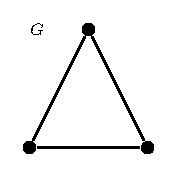
\includegraphics[scale = 0.8]{fig45.pdf}
\end{center}

Dann gilt $m(G)=1$ und $c(G)=2$. \\ \vspace*{0.2cm}

Das Beispiel zeigt, dass $m(G) < c(G)$ für nichtbipartite Graphen möglich ist. 
\end{frame}

\begin{frame}
 \frametitle{Satz von König}
 Für bipartite Graphen gilt dagegen der folgende \alert{Satz von König}\footnote{Dénes König (1884-1944), ungarischer Mathematiker.}. \\ \vspace*{0.2cm}
 
 \textbf{Satz (D. König, 1931):} Für jeden bipartiten Graphen gilt
\begin{equation}
\label{eq:11:2}
m(G) = c(G).
\end{equation}

Wir werden einen \alert{konstruktiven Beweis des Satzes von König} geben: \alert{Der Beweis wird eine Methode liefern, wie man in einem bipartiten Graphen eine minimale Knotenüberdeckung findet}. \\ \vspace*{0.2cm}

Wenn man in einem bipartiten Graphen ein Matching $M$ mit maximaler Kantenzahl gefunden hat, \alert{so ist es sehr nützlich, gleichzeitig auch eine minimale Knotenüberdeckung $U$, also eine Knotenüberdeckung mit $|U|=|M|$ zu besitzen}.
\end{frame}

\begin{frame}
 \frametitle{Zertifikat und Verifikation}
 Stellen Sie sich vor, Sie haben in mühevoller Rechnung für einen sehr großen bipartiten Graphen ein Matching $M$ mit maximaler Kantenzahl gefunden. Dem Matching selbst kann man dann in der Regel nicht ansehen, dass es kein Matching mit größerer Kantenzahl gibt. \\ \vspace*{0.2cm}
 
 Wenn Sie aber gleichzeitig eine Knotenüberdeckung $U$ präsentieren, für die $|U|=|M|$ gilt, so wird jeder sofort einsehen, dass es sich bei $M$ in der Tat um ein Matching mit maximaler Kantenzahl handelt. \\ \vspace*{0.2cm}
 
 Die Knotenüberdeckung $U$ ist in diesem Fall ein hervorragendes Mittel, um die Optimalität von $M$ zu \alert{verifizieren}. Anders gesagt: $U$ ist ein \alert{Zertifikat} für die Optimalität von $M$.
\end{frame}

\begin{frame}
 \frametitle{Beweis des Satzes von König}
 Der im Folgenden präsentierte konstruktive Beweis des Satzes von König knüpft an unseren Algorithmus zum Auffinden eines Matchings mit maximaler Kantenzahl an. Eine zentrale Rolle spielt dabei der Begriff des \alert{alternierenden Pfades}, den wir im vorangegangenen Abschnitt kennengelernt haben. \\ \vspace*{0.2cm}

\textbf{Beweis des Satzes von König}\index{Beweis!des Satzes von König}\index{König, Satz von! Beweis}. $G$ sei bipartit. Zu zeigen ist $m(G) = c(G)$. Es sei $M$ ein Matching von $G$ mit $|M|=m(G)$. Zu finden ist eine Knotenüberdeckung $U$ von $G$ mit $|U|=|M|$. Wie üblich bezeichnen wir mit $X$ und $Y$ eine zu $G$ gehörige Knotenpartition. \\ \vspace*{0.2cm}

Mit $S$\label{page:11:7} bezeichnen wir die Menge derjenigen Knoten von $G$, die von $X$ aus mit einem alternierenden Pfad\index{alternierender Pfad}\index{Pfad!alternierender} erreichbar sind. (Zur Erinnerung: Ein alternierender Pfad startet immer in einem ungepaarten Knoten von $X$.) 
\end{frame}

\begin{frame}
 \frametitle{Definition von $U$}
 Es sei
\[
U := \big( X \setminus S \big) \cup \big( Y \cap S \big).
\]

\begin{center}
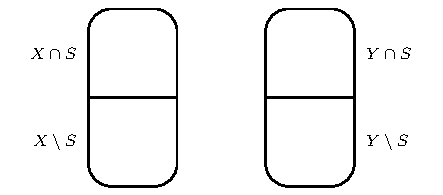
\includegraphics[scale=0.8]{fig46.pdf}
\end{center}

Es gelten die folgenden Feststellungen:
\begin{enumerate}[i)]
\item In $X \setminus S$ gibt es keine ungepaarten Knoten (nach Definition von $S$ und aufgrund der Tatsache, dass ein ungepaarter Knoten $x \in X$ für sich allein genommen bereits einen alternierenden Pfad darstellt).
\item In $Y \cap S$ gibt es ebenfalls keine ungepaarten Knoten (, da es sonst einen augmentierenden Pfad gäbe, im Widerspruch zu $|M|=m(G)$).
\item Es gibt keine Kante aus $M$, die $Y \cap S$ mit $X \setminus S$ verbindet (, da es sonst einen alternierenden Pfad gäbe, der einen Knoten aus $X \setminus S$ erreicht).
\end{enumerate}

\end{frame}

\begin{frame}
 \frametitle{Nachweis von $|U| \le |M|$}
 Aus i)--iii) folgt, dass sämtliche Knoten aus $U$ auf Kanten aus $M$ liegen, und zwar je zwei verschiedene Knoten von $U$ auf unterschiedlichen Kanten aus $M$. Es folgt
\[
|U| \leq |M|.
\]

Darüber hinaus gilt: 
\begin{enumerate}[i)]
\addtocounter{enumi}{3}
\item Es gibt keine Kanten zwischen $X \cap S$ und $Y \setminus S$.
\end{enumerate} \vspace*{0.2cm}

\textbf{Begründung zu iv):} Angenommen, $e=\bigl\{ x',y' \bigr\}$ wäre eine Kante von $G$ mit $x' \in X \cap S$ und $y' \in Y \setminus S$. Wegen $x' \in X \cap S$ existiert ein alternierender Pfad $P$, der in $x'$ endet. Dann folgt:
\begin{itemize}
\item Dann ist $P$ entweder nur einpunktig (d.h., $x'$ ist ein ungepaarter Knoten);
\item oder $P$ durchläuft abwechselnd Knoten aus $X \cap S$ und $Y \cap S$, wobei sich Nicht-Matchingkanten und Matchingkanten abwechseln und die letzte Kante eine Matchingkante ist. 
\end{itemize}
\alert{In beiden Fällen würde $e \notin M$ gelten und $y'$ wäre durch einen alternierenden Pfad erreichbar, im Widerspruch zu $y' \notin S$.}
\end{frame}

\begin{frame}
 \frametitle{$U$ ist eine Knotenüberdeckung mit $|U| = |M|$}
 Feststellung iv) bedeutet, dass $U$ eine Knotenüberdeckung von $G$ ist, weshalb insbesondere $|U| \geq |M|$ gilt. Oben hatten wir bereits $|U| \leq |M|$ festgestellt. Insgesamt haben wir also (wie gewünscht) eine Knotenüberdeckung $U$ mit $|U| = |M|$ erhalten. \qquad $\Box$ \\ \vspace*{0.2cm}
 
 Wir kommen nun zurück auf unseren Matching-Algorithmus für bipartite Graphen $G=(V,E)$ mit Knotenpartition $V=X \cup Y$. \\ \vspace*{0.2cm}
 
 In diesem wurde auf das zu $G$ gehörige Netzwerk $N=(G',c,s,t)$ der Algorithmus von Edmonds und Karp angewandt. (Zur Definition von $N$ siehe Folie \pageref{page:11:6}.) \alert{Es sei $(S',T')$ der vom Algorithmus von Edmonds und Karp gelieferte minimale Schnitt von $N=(G',c,s,t)$.}
\end{frame}

\begin{frame}
 \frametitle{Wie man eine minimale Knotenüberdeckung erhält}
 Vergleicht man den Beweis des Max-Flow-Min-Cut-Theorems mit dem Beweis des Satzes von König, so erkennt man, dass für die im Beweis des Satzes von König definierte Menge $S$ gilt: $S = S' \setminus \big\{ s \big\}$. (Um zu erkennen, dass dies tatsächlich so ist, beachte man vor allem die Feststellung, dass ein Knoten $w$ in $G$ genau dann mit einem alternierenden Pfad erreichbar ist, wenn er in $N$ mit einem zunehmenden Pfad erreichbar ist.) \\ \vspace*{0.2cm}

\alert{Damit ist klar, dass unser Matching-Algorithmus für bipartite Graphen nicht nur ein Matching \index{maximales Matching}\index{Matching!maximales} $M$ mit maximaler Kantenzahl, sondern auch eine minimale Knotenüberdeckung $U$ liefert, die man wie folgt bekommt}: Ist $(S',T')$ der gefundene minimale Schnitt von $N=(G',c,s,t)$, so sei $S = S' \setminus \big\{ s \big\}$. Dann gilt:
\begin{equation*}
%\label{eq:11:3}
U = \big( X \setminus S \big) \cup \big( Y \cap S \big).
\end{equation*}
\end{frame}

\begin{frame}
 \frametitle{Zwei Beispiele}
 In diesem Abschnitt wird der zuvor besprochene Matching-Algorithmus anhand von zwei Beispielen illustriert. 
 \begin{itemize}
 \item Im ersten Beispiel wird die Vorgehensweise sehr detailliert beschrieben, wobei zwischendurch auch immer das zum Graphen $G$ gehörende Netzwerk $N=(G',c,s,t)$ betrachtet wird.
 \item Im zweiten Beispiel wird dann (wie allgemein üblich) das Netzwerk $N$ überhaupt nicht mehr herangezogen: \alert{Das Vorgehen wird nur noch in der Sprache der ungerichteten Graphen, Matchings und alternierenden Pfade beschrieben.}
 \end{itemize}
\end{frame}

\begin{frame}
 \frametitle{Beispiel 1}
 Wir betrachten den folgenden bipartiten Graphen $G=(V,E)$ mit $V = X \cup Y$ für $X = \big\{ x_1,x_2,x_3,x_4 \big\}$ und $Y = \big\{ y_1,y_2,y_3 \big\}$:

\begin{center}
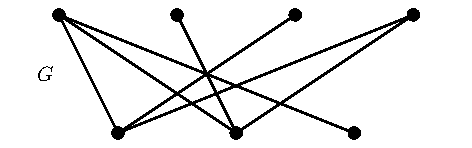
\includegraphics{fig47.pdf}
\end{center}

Die \textbf{Aufgabe} ist, ein Matching mit maximaler Kantenzahl und gleichzeitig eine minimale Knotenüberdeckung zu finden. Hierzu soll der Algorithmus von Edmonds und Karp verwendet werden, wobei die \alert{folgende Regel} zu beachten ist:
\begin{center}
\begin{tabular}{rl}
& Ist im Algorithmus von Edmonds und Karp die Reihenfolge der zu  \\
($\star$)    & markierenden Knoten nicht festgelegt, \alert{\textit{so sind Knoten mit kleinerem}} \\
    & \alert{\textit{Index vorzuziehen.}}
\end{tabular}
\end{center}
\end{frame}


\begin{frame}
 \frametitle{Das Netzwerk $N$}
 Wir verwandeln als erstes den bipartiten Graphen $G$ in ein Netzwerk $N=(G',c,s,t)$:
 \begin{center}
  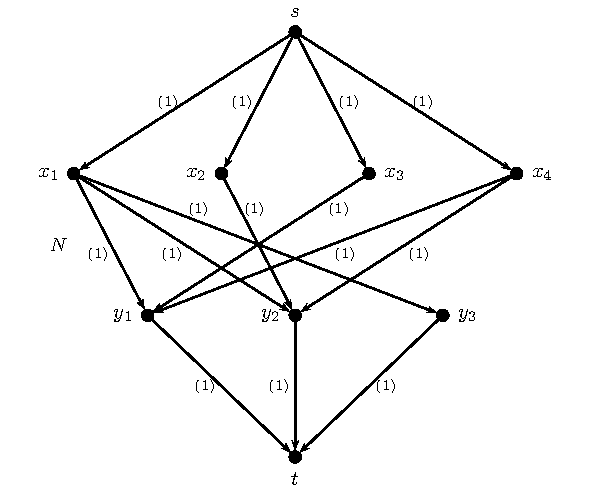
\includegraphics[scale = 0.8]{fig48.pdf}
 \end{center}
\end{frame}

\begin{frame}
 \frametitle{Vergabe der Markierungen}
 Los geht es wie immer mit dem Nullfluss, den wir $f_0$ nennen wollen. In  Abbildung~\ref{abb:11:1} sind außerdem die Markierungen eingetragen, die vom Algorithmus vergeben werden, bevor es zur ersten Flussvergrößerung kommt: \\ \vspace*{0.2cm}
 
 Die Knoten wurden in der Reihenfolge $s,x_1,x_2,x_3,x_4,y_1,y_2,y_3,t$ markiert. Diese Reihenfolge ergibt sich aus Zeile (5') des Algorithmus von Edmonds und Karp ({\glqq}first labelled -- first scanned{\grqq}) sowie aus der obigen Regel ($\star$).
\end{frame}

\begin{frame}
 \frametitle{Vergabe der Markierungen}
 \begin{figure}
 \begin{center}
  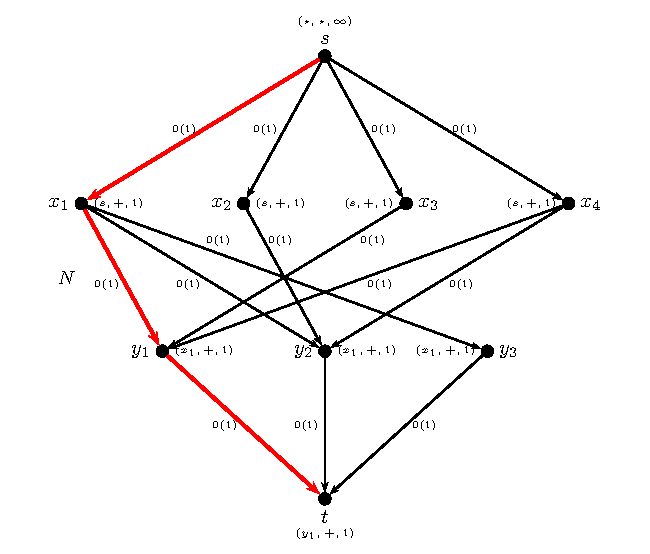
\includegraphics[scale = 0.72]{fig49.pdf}
 \end{center}
 \caption{Der erste flussvergrößernde Pfad}
 \label{abb:11:1}
 \end{figure}
\end{frame}

\begin{frame}
 \frametitle{Der verbesserte Fluss}
 Der gefundene flussvergrößernde Pfad $P'=(s,x_1,y_1,t)$ wurde in Abbildung \ref{abb:11:1} fett eingezeichnet; der verbesserte Fluss, den wir $f_1$ nennen wollen, wurde weiter unten in Abbildung \ref{abb:11:3} eingetragen. Es gilt
\begin{align*}
f_1(s,x_1) &= 1, \\
f_1(x_1,y_1) &= 1, \\
f_1(y_1,t) &= 1,
\end{align*}
und $f_1(e)=0$ für alle übrigen Kanten des Netzwerks $N$. Das Ergebnis der ersten Flussvergrößerung ist, dass wir den Fluss $f_0$ zu $f_1$ verbessert haben. Übertragen wir dieses Ergebnis auf den bipartiten Graphen $G$, so können wir feststellen: 
\end{frame}

\begin{frame}
 \frametitle{Das aktuelle Matching}
  \alert{Am Anfang waren noch keine Matchingkanten vorhanden und nach der ersten Flussvergrößerung besteht das aktuelle Matching aus genau einer Kante, nämlich der Kante $\big\{ x_1,y_1 \big\}$}:
 \begin{center}
  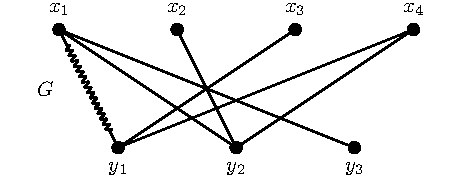
\includegraphics{fig50.pdf}
 \end{center}
In Abbildung \ref{abb:11:3} sind neben dem Fluss $f_1$ die Markierungen eingetragen, die vom Algorithmus vergeben werden, bevor es zur Verbesserung von $f_1$ kommt; dabei wurden die Knoten in der Reihenfolge $s,x_2,x_3,x_4,y_2,y_1,t$ markiert. Als flussvergrößernden Pfad erhält man $P'=(s,x_2,y_2,t)$.
\end{frame}

\begin{frame}
 \frametitle{Ein weiterer flussvergrößernder Pfad}
 \begin{figure}
  \begin{center}
   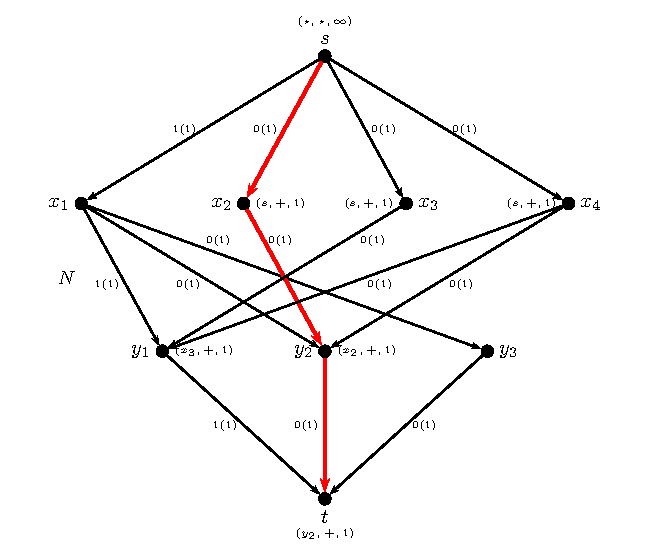
\includegraphics[scale = 0.72]{fig51.pdf}
  \end{center}
  \caption{Ein weiterer flussvergrößernder Pfad}
  \label{abb:11:3}
 \end{figure}

\end{frame}

\begin{frame}
 \frametitle{Das aktuelle Matching}
 Verbesserung von $f_1$ mittels $P'$ führt zum Fluss $f_2$ (wie in Abbildung \ref{abb:11:5} angegeben) sowie zum Matching $M_2 = \big\{ \{x_1,y_1\}, \{x_2,y_2\} \big\}$:

\begin{center}
 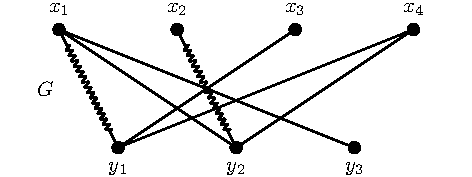
\includegraphics{fig52.pdf}
\end{center}
\end{frame}

\begin{frame}
 \frametitle{Der bisherige Verlauf}
 Bezeichnen wir mit $M_0$ die leere Menge sowie mit $M_1$ das Matching, das nach der ersten Flussvergrößerung aktuell war, so können wir den bisherigen Verlauf wie folgt darstellen:
\[
\begin{array}{ccl}
f_0 & & M_0 = \emptyset \\
\downarrow & & \ \downarrow \\
f_1 & & M_1 = \big\{ \{x_1,y_1 \} \big\} \\
\downarrow & & \ \downarrow \\
f_2 & & M_2 = \big\{ \{x_1,y_1 \}, \{x_2,y_2\} \big\} \\
\end{array}
\]

Alles was bislang passiert ist, lässt sich wie folgt in einem einzigen Satz zusammenfassen:

\begin{center}
\alert{In den ersten beiden Iterationen wählt der Algorithmus die \\
Kanten $\big\{ x_1,y_1 \big\}$ und $\big\{ x_2,y_2 \big\}$ als Matchingkanten aus.}
\end{center}
\end{frame}

\begin{frame}
 \frametitle{Die 3. Iteration}
  Nun geht es in die nächste Runde (3. Iteration): \\ \vspace*{0.2cm}
  
  Es werden Markierungen wie in Abbildung \ref{abb:11:5} vergeben, wobei die Knoten in folgender Reihenfolge markiert werden: $s,x_3,x_4,y_1,y_2,x_1,x_2,y_3,t$. Dies führt zu folgendem Ergebnis (siehe z.B. Abbildungen \ref{abb:11:5} und \ref{abb:11:6}):
  \begin{itemize}
  \item in $N$ zum \alert{flussvergrößernden Pfad} $P'=(s,x_3,y_1,x_1,y_3,t)$;
  \item in $G$ zum \alert{augmentierenden Pfad} $P=(x_3,y_1,x_1,y_3)$.
  \end{itemize}
\end{frame}

\begin{frame}
 \frametitle{Ein weiterer flussvergrößerender Pfad}
\begin{figure}[H]
\begin{center}
 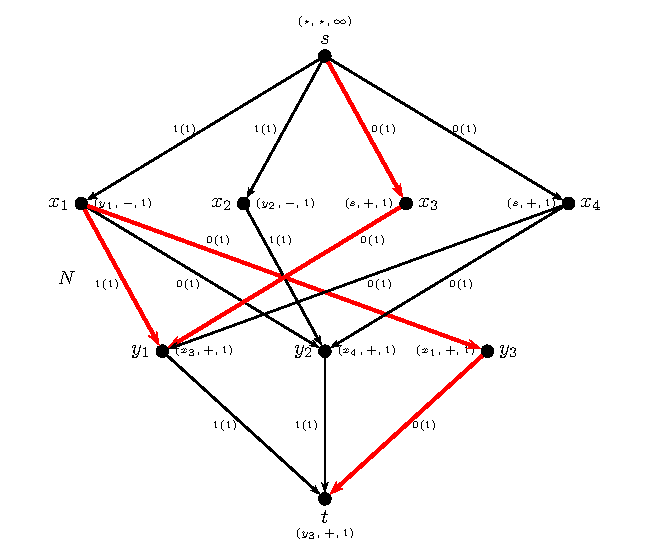
\includegraphics[scale=0.72]{fig53.pdf}
\end{center}
\caption{Der flussvergrößernde Pfad $P'=(s,x_3,y_1,x_1,y_3,t)$.}
\label{abb:11:5}
\end{figure}
\end{frame}

\begin{frame}
\frametitle{Austausch von Matching- und Nicht-Matchingkanten}
\begin{figure}[H]
\begin{center}
 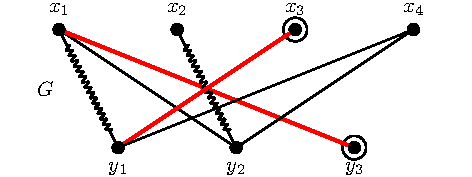
\includegraphics{fig54.pdf}
\end{center}
\caption{Der augmentierende Pfad $P=(x_3,y_1,x_1,y_3)$.}
\label{abb:11:6}
\end{figure}

Der Austausch von Nicht-Matchingkanten und Matchingkanten von $P$ führt zum Matching
\[
M_3 = \big\{ \{x_1,y_3\}, \{x_2,y_2\}, \{x_3,y_1\} \big\},
\]

das in der folgenden Darstellung wiedergegeben wird:
\end{frame}

\begin{frame}
\frametitle{Das Matching $M_3$}
\begin{center}
 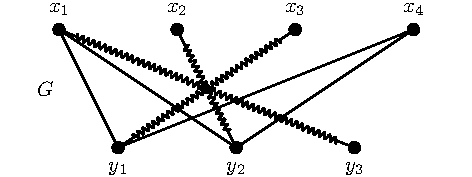
\includegraphics{fig55.pdf}
\end{center}
\end{frame}

\begin{frame}
 \frametitle{Die 4. und letzte Iteration}
 Nun geht es -- wie man sich bereits denken kann -- in die letzte Runde (4.~Iteration), in der der Algorithmus kein verbessertes Matching findet, stattdessen aber ein \alert{Zertifikat für die Optimalität von $M_3$} liefert. Der Abbildung \ref{abb:11:8} entnimmt man, welche Knoten markiert werden; die Markierung erfolgt dabei in der Reihenfolge 
 $$s,x_4,y_1,y_2,x_3,x_2.$$
 Die übrigen Knoten werden nicht markiert, da sie nicht durch einen zunehmenden Pfad erreicht werden. \\ \vspace*{0.2cm}
 Man erhält den Schnitt $(S',T')$ mit $S'=\bigl\{ s,x_2,x_3,x_4,y_1,y_2 \bigr\}$ und $T'=\bigl\{ x_1,y_3,t \bigr\}$.
\end{frame}

\begin{frame}
 \frametitle{Der Schnitt $(S',T')$}
\begin{figure}[H]
\begin{center}
 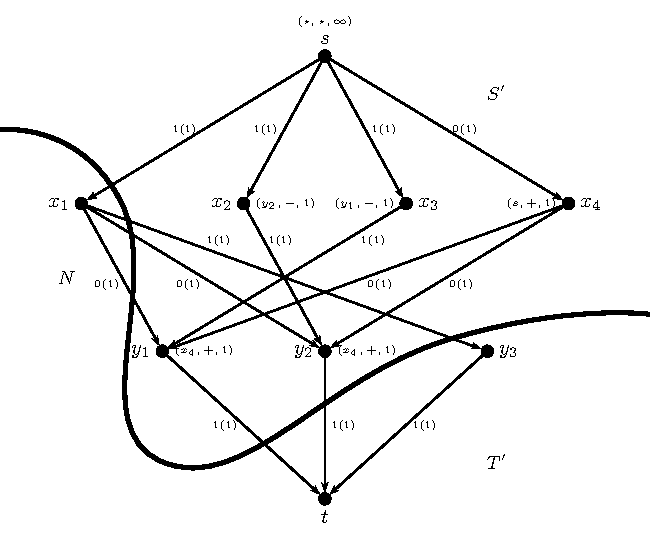
\includegraphics[scale=0.72]{fig56.pdf}
\end{center}
\caption{Der Schnitt $(S',T')$.}
\label{abb:11:8}
\end{figure}
\end{frame}


\end{document}
